\documentclass[11pt,border=5pt]{standalone}
\usepackage{fontspec}
\setmainfont{cmunrm.otf}[BoldFont=cmunbx.otf,ItalicFont=cmunti.otf,BoldItalicFont=cmunbi.otf]
\usepackage{amsmath}
\usepackage{unicode-math}
\setmathfont{NewCMMath-Regular.otf}
\usepackage{tikz}
\usetikzlibrary{arrows.meta,patterns,angles,quotes}
\begin{document}
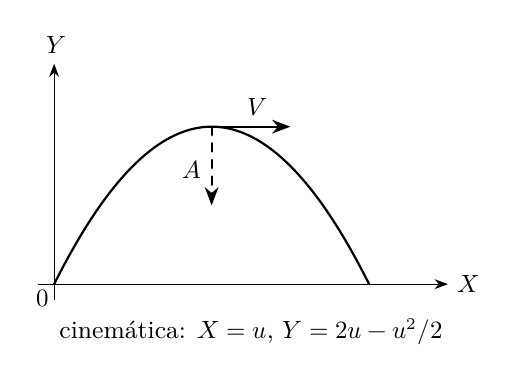
\begin{tikzpicture}[>=Stealth,font=\small,line cap=round,line join=round]
\draw[->,thin] (-0.2,0) -- (5,0) node[pos=1,right] {$X$};
\draw[->,thin] (0,-0.2) -- (0,2.8) node[pos=1,above] {$Y$};
\node at (-0.14,-0.18) {$0$};
\draw[thick] plot coordinates {(0.00000,0.00000) (0.03333,0.06611) (0.06667,0.13111) (0.10000,0.19500) (0.13333,0.25778) (0.16667,0.31944) (0.20000,0.38000) (0.23333,0.43944) (0.26667,0.49778) (0.30000,0.55500) (0.33333,0.61111) (0.36667,0.66611) (0.40000,0.72000) (0.43333,0.77278) (0.46667,0.82444) (0.50000,0.87500) (0.53333,0.92444) (0.56667,0.97278) (0.60000,1.02000) (0.63333,1.06611) (0.66667,1.11111) (0.70000,1.15500) (0.73333,1.19778) (0.76667,1.23944) (0.80000,1.28000) (0.83333,1.31944) (0.86667,1.35778) (0.90000,1.39500) (0.93333,1.43111) (0.96667,1.46611) (1.00000,1.50000) (1.03333,1.53278) (1.06667,1.56444) (1.10000,1.59500) (1.13333,1.62444) (1.16667,1.65278) (1.20000,1.68000) (1.23333,1.70611) (1.26667,1.73111) (1.30000,1.75500) (1.33333,1.77778) (1.36667,1.79944) (1.40000,1.82000) (1.43333,1.83944) (1.46667,1.85778) (1.50000,1.87500) (1.53333,1.89111) (1.56667,1.90611) (1.60000,1.92000) (1.63333,1.93278) (1.66667,1.94444) (1.70000,1.95500) (1.73333,1.96444) (1.76667,1.97278) (1.80000,1.98000) (1.83333,1.98611) (1.86667,1.99111) (1.90000,1.99500) (1.93333,1.99778) (1.96667,1.99944) (2.00000,2.00000) (2.03333,1.99944) (2.06667,1.99778) (2.10000,1.99500) (2.13333,1.99111) (2.16667,1.98611) (2.20000,1.98000) (2.23333,1.97278) (2.26667,1.96444) (2.30000,1.95500) (2.33333,1.94444) (2.36667,1.93278) (2.40000,1.92000) (2.43333,1.90611) (2.46667,1.89111) (2.50000,1.87500) (2.53333,1.85778) (2.56667,1.83944) (2.60000,1.82000) (2.63333,1.79944) (2.66667,1.77778) (2.70000,1.75500) (2.73333,1.73111) (2.76667,1.70611) (2.80000,1.68000) (2.83333,1.65278) (2.86667,1.62444) (2.90000,1.59500) (2.93333,1.56444) (2.96667,1.53278) (3.00000,1.50000) (3.03333,1.46611) (3.06667,1.43111) (3.10000,1.39500) (3.13333,1.35778) (3.16667,1.31944) (3.20000,1.28000) (3.23333,1.23944) (3.26667,1.19778) (3.30000,1.15500) (3.33333,1.11111) (3.36667,1.06611) (3.40000,1.02000) (3.43333,0.97278) (3.46667,0.92444) (3.50000,0.87500) (3.53333,0.82444) (3.56667,0.77278) (3.60000,0.72000) (3.63333,0.66611) (3.66667,0.61111) (3.70000,0.55500) (3.73333,0.49778) (3.76667,0.43944) (3.80000,0.38000) (3.83333,0.31944) (3.86667,0.25778) (3.90000,0.19500) (3.93333,0.13111) (3.96667,0.06611) (4.00000,0.00000)};
\draw[->,thick] (2,2) -- (3,2) node[pos=0.55,above] {$V$};
\draw[->,thick,dashed] (2,2) -- (2,1) node[pos=0.55,left] {$A$};
\node at (2.5,-0.6) {cinemática: $X=u$, $Y=2u-u^2/2$};

\end{tikzpicture}
\end{document}
